\documentclass[fontsize=11pt]{article}
\usepackage{amsmath}
\usepackage[utf8]{inputenc}
\usepackage[margin=0.75in]{geometry}
\usepackage{graphicx}
\usepackage{hyperref}
\usepackage{url}
\usepackage{xurl}
\hypersetup{
    colorlinks=true,
    linkcolor=blue,
    filecolor=magenta,      
    urlcolor=cyan,
    pdftitle={Overleaf Example},
    pdfpagemode=FullScreen
}

\title{
CSC110 Project Proposal:  \\
The Impact of Covid-19 on the Financial Markets.
}
\author{Selina Phadiya, Natasha Sharan, Lily Su, Seyoung Yoo}
\date{Friday, November 5, 2021}

\begin{document}
\maketitle

\section*{Problem Description and Research Question}
\textbf{Research question: \\
\\
\lq\lq How much did Covid-19 impact the financial markets, and did it impact some markets more than others?"} \\\\
\emph{Background Information} \\
The objective of this project is to analyse the impact of Covid-19 on benchmark index funds, thus having an understanding about them is essential.
An index fund is a statistical tool designed to match or track the components of a financial market.
All index funds are developed for a variety of purposes and objectives (Fernando). A benchmark index is an index which serves as a standard by which other stock’s performance can be measured (Chen). An example of a benchmark is S\&P 500 which measures the United States’ market performance by following the 500 largest companies which trade on NYSE, Nasdaq, or Cboe. \\ \\
\emph{Context of the Problem} \\
The COVID-19 pandemic has severely disrupted the financial markets worldwide. At its roots, COVID-19 crisis is not a financial or economic crisis; it is a health crisis. However, its impact on supply and demand chain has resulted in the pandemic turning into a large-scale financial and economical crisis. Hence, it is extremely important to understand and analyse the global economic and financial state (Bradley).\\
In order to understand the financial impact, we need to get to the roots of the market crash. Hence, our research question revolves around how much was each market impacted. We decided to analyse the benchmark indexes, because the stock market provides a unique way to view and predict the global economy as it is based on the value of firms (\lq\lq Impact of COVID-19 on the Global Financial Markets - Statistics \& Facts").\\
In conclusion, we have selected the top 5 major index funds, and after a thorough analysis we would be able to conclude the followings things:
\begin{enumerate}
\setcounter{enumi}{0}
\item How much was each country’s index fund impacted by Covid-19?
\item How many countries’ index funds price exceeded the pre-pandemic prices?
\item How many countries’ index funds are still undervalued? \\
\end{enumerate}
\emph{Why We Chose to Explore the Impact of Covid-19 on Benchmark Index Funds?} \\
COVID-19 severely disrupted people’s lifestyles. Therefore, the topic of life after the pandemic piqued our group’s interest. Recovery from economic recession during COVID-19 will be in progress after restrictions lift. As a result, we chose to focus on companies’ financial stability relating to their ability to continue their production of goods post-pandemic. Evaluating companies’ stocks is a reliable way to measure companies’ financial stability. However, considering the stock for every company is impossible because thousands of companies are present on a stock exchange. Therefore, we chose to analyze different countries’ benchmark index funds (Bradley).
\pagebreak



\section*{Dataset Description}

\emph{Sample Data for Covid-19 Cases} \\
Figure 1 is a small sample from one of our datasets which contain all countries and their Covid-19 cases reported daily. The format of the dataset is an excel file and we are going to filter the data so that it only includes countries with the biggest benchmark index funds (UK, Japan, US, Brazil, India, France). This dataset is produced by Our World in Data and is completely open access under the 
\href{https://creativecommons.org/licenses/by/4.0/}{Creative Commons BY license}.
On their GitHub repository, the dataset is available via the following link, 
\href{https://github.com/owid/covid-19-data/tree/master/public/data}{https://github.com/owid/covid-19-data/tree/master/public/data} and specifically this
\href{https://covid.ourworldindata.org/data/owid-covid-data.xlsx}{link} allows direct access to the excel file.
\begin{figure}[htp]
    \centering
    \includegraphics[width=10cm]{covid_data.png}
    \caption{A screenshot of our sample data of Covid-19 cases in the United States.}
    \label{fig:stock}
\end{figure}
\\\\\emph{Sample Data for Benchmark Index Funds}\\
Figure 2 displays the historical data for S\&P 500. It has several entities that are not relevant to our analysis, thus we will implement algorithms to filter the data. The raw data for the five countries of focus can be found through the following links:
\href{https://ca.finance.yahoo.com/quote/\%5EGSPC/history?period1=1546387200&period2=1622592000&interval=1wk&filter=history&frequency=1wk&includeAdjustedClose=true}{United States}, 
\href{https://ca.finance.yahoo.com/quote/\%5EBSESN/history?period1=1546300800&period2=1622505600&interval=1wk&filter=history&frequency=1wk&}{India}, 
\href{https://finance.yahoo.com/quote/\%5EBVSP/history?period1=1546387200&period2=1622592000&interval=1wk&filter=history&frequency=1wk&includeAdjustedClose=true}{Brazil}, 
\href{https://ca.finance.yahoo.com/quote/\%5EN225/history?period1=1546300800&period2=1622505600&interval=1d&filter=history&frequency=1d&includeAdjustedClose=true}{Japan}, 
\href{https://finance.yahoo.com/quote/\%5EFCHI/history?period1=1546646400&period2=1622505600&interval=1wk&filter=history&frequency=1wk&includeAdjustedClose=true}{France}.

\begin{figure}[htp]
    \centering
    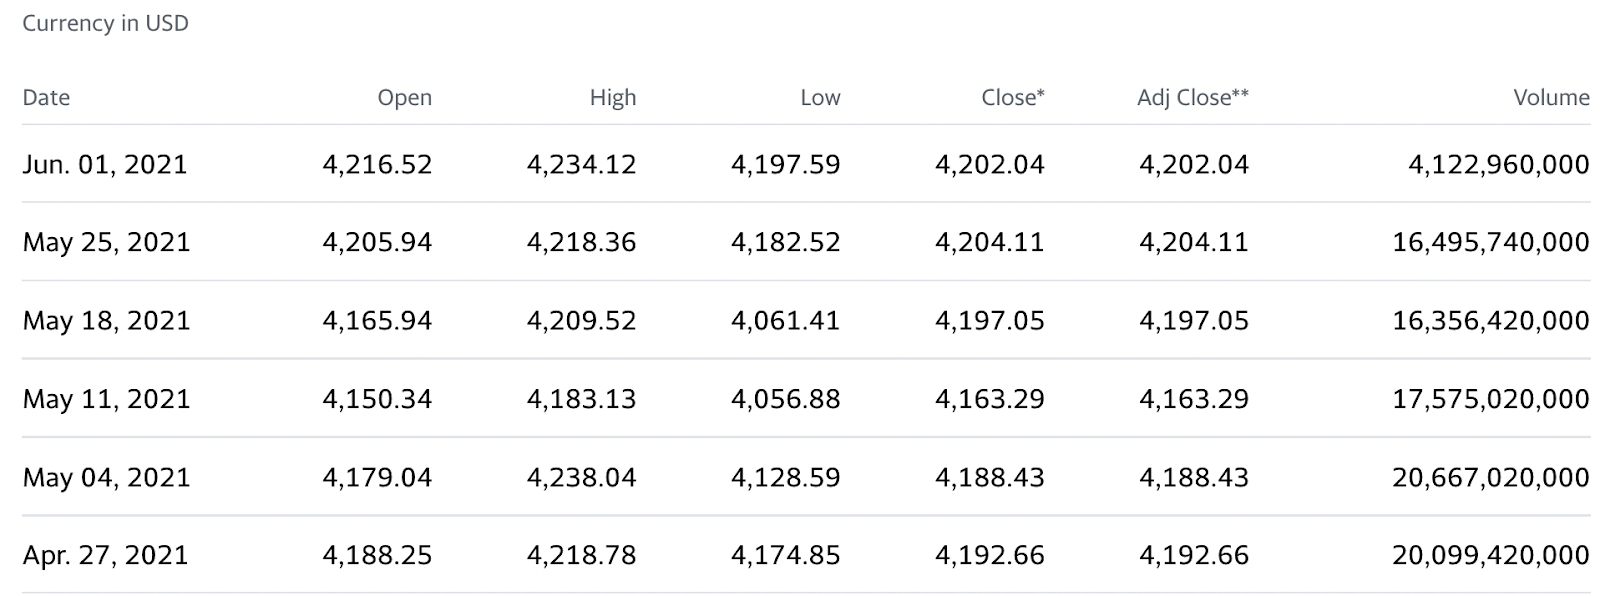
\includegraphics[width=14cm]{us_stock_data.png}
    \caption{A screenshot of our sample data of a benchmark index fund (S\&P500).}
    \label{fig:stock}
\end{figure}
\pagebreak

\section*{Computational Plan}

\emph {Stage 1: Filtering to Clean the Data}


\begin{enumerate}
\setcounter{enumi}{0}
\item Our raw data for Covid-19 cases contain irrelevant information like total cases per million and new cases per million. Similarly, the raw data for benchmark index fund price contains irrelevant data like opening costs. Thus, algorithms will be used to filter and clean our raw data for our relevant use, and also help perform simple calculations. \\
\end{enumerate}
\emph{Stage 2: Transforming the Data}
\begin{enumerate}
\setcounter{enumi}{0}
\item The price of benchmark index funds, from our raw data, is available in weekly intervals. Calculate the weekly average of new Covid cases for each country.
\item Since we are comparing index funds with different currencies, we will use a method to take the date, currency, closing price of the index fund, and the conversion rate (on that date) and return the price of that index fund in USD.
\item Implement sorting algorithms to order the data appropriately.\\
\end{enumerate}
\emph{Stage 3: Performing Computational Analysis on the Data}
\begin{enumerate}
\setcounter{enumi}{0}
\item The 2020 stock market crash occurred among the dates of 20 February 2020 - 07 April 2020 (\lq\lq 2020 Stock Market Crash - Wikipedia"). Calculate percentage loss of the index fund between 19 February 2020 (pre-pandemic) and the lowest it reached during the market crash.
\item Calculate the mean and median of the list of percentage changes of the benchmark index funds’ closing price.
\item Calculate the standard deviation to see how relevant the mean is to the rest of the data. Precisely, to see how tightly clustered the mean percent is to the other percentages. 
\item The correlation coefficient (R²) will be calculated to quantify how correlated the number of covid cases and the stock index fund values are. The closer the value is to 1, the stronger the correlation.
\item Check whether the closing price of the index funds reached or surpassed the closing price they had before the market crash (19 February 2020). If the index fund recovered, calculate the number of months it took to recover.\\
\end{enumerate}
\emph{Stage 4: Presenting the Data}\\
We are going to represent our data and the analysis we performed on it using the four graphs:
\begin{enumerate}
\setcounter{enumi}{0}
\item Choropleth World map to present how many countries’ index funds recovered and exceeded their pre-pandemic closing price. 
\item Line Graph to plot all 5 index funds closing price against time. 
\item Line Graph to plot the benchmark index fund price and the number of Covid cases against time.
\item Scatter Plot to present the correlation between number of Covid cases and drop in the index funds’ price (\%).
\item Table to show recovery (\%) of each index fund over time (e.g. 1 week, 1 month, 3 month, 6 month, 1 year).\\
\end{enumerate}
\emph{Technical Requirement}\\
Our project will be relying on some libraries to perform certain tasks. Some of these include numpy, pygame, pandas, plotly.express, plotly.graph\_obj and CurrencyConverter. To elaborate on the usage of NumPy, it provides a variety of mathematical functions. It’s usage is significant as data analysis and performing calculations will compose a large portion of this project. We will use numpy.mean(), numpy.median(), and numpy.std(). All three functions take a list as a parameter. numpy.mean() returns the mean value. numpy.median() returns the median value. numpy.std() returns the standard deviation.
\pagebreak

\section*{References}
% NOTE: LaTeX does have a built-in way of generating references automatically,
% but it's a bit tricky to use so we STRONGLY recommend writing your references
% manually, using a standard academic format like APA or MLA.
% (E.g., https://owl.purdue.edu/owl/research_and_citation/apa_style/apa_formatting_and_style_guide/general_format.html)


“CAC 40 (\textasciicircum FCHI) Historical Data.” Yahoo! Finance, Yahoo!, 5 Nov. 2021,\\ {https://finance.yahoo.com/quote/\%5EFCHI/history?period1=1546646400\&period2=1622505600
\&interval=1wk\&filter=\\history 
\&frequency=1wk\&includeAdjustedClose=true}
\newline 
\\
“IBOVESPA (\textasciicircum BVSP) Historical Data.”  Yahoo! Finance, Yahoo!, 5 Nov. 2021,\\
https://finance.yahoo.com/quote/\%5EBVSP/history?period1=1546387200\&period2=1622592000
\&interval=1wk\\\&filter=history\&frequency=1wk\&includeAdjustedClose=true\\ 
\\
“Nikkei 225 (\textasciicircum N225) Historical Data.” Yahoo! Finance, Yahoo!, 5 Nov. 2021, \\
https://ca.finance.yahoo.com/quote/\%5EN225/history?period1=1546300800\&period2=1622505600
\&interval=1d\&filter\\
=history\&frequency=1d\&includeAdjustedClose=true.\\ 
\\
“S\&P BSE SENSEX (\textasciicircum BSESN) Historical Data.” Yahoo! Finance, Yahoo!, 5 Nov. 2021,\\
https://ca.finance.yahoo.com/quote/\%5EBSESN/history?period1=1546300800\&period2=1622505600\&interval\\=1wk\&filter=history\&frequency=1wk\&
\\
\\
“S\&P 500 (\textasciicircum GSPC) Historical Data” Yahoo! Finance, Yahoo!, 5 Nov. 2021,\\
https://ca.finance.yahoo.com/quote/\%5EGSPC/history?\\period1=1546387200\&period2=1622592000
\&interval=1wk\&filter=history\&frequency=1wk\&includeAdjustedClose=true.
\\
\\
Nytimes. “Covid-19-Data/Us.Csv at Master · Nytimes/Covid-19-Data · GitHub.” Github,\\ https://github.com/nytimes/covid-19-data/blob/master/us.csv. Accessed 5 Nov. 2021.
\\ 
\\
Gupta, Mohit. “Numpy.Std() in Python - GeeksforGeeks.” GeeksforGeeks, 28 Nov. 2018,https://www.geeksforgeeks.org/\\
numpy-std-in-python/.
\\
\\
“Mathematical Functions — NumPy v1.21 Manual.” NumPy, 2021, https://numpy.org/doc/stable/reference/routines.\\
math.html.
\\
\\
Sharma, Palash. “Tutorial - Numpy Mean, Numpy Median, Numpy Mode, Numpy Standard Deviation in Python - MLK - Machine Learning Knowledge” MLK - Machine Learning Knowledge, 
https://machinelearningknowledge.ai/tutorial-numpy-mean-numpy-median-numpy-mode-numpy-standard-deviation-in-python/.
\\
\\
“Plotly Python Graphing Library | Python | Plotly.” Plotly: The Front End for ML and Data Science Models, https://plotly.com/python/.
\\
\\
Stephanie Glen. “Correlation Coefficient: Simple Definition, Formula, Easy Steps” From StatisticsHowTo.com: Elementary Statistics for the rest of us! https://www.statisticshowto.com/probability-and-statistics/correlation-coefficient-formula/.
\\
\\
Mathieu, Edouard, Sheet of Newt. Newt Fanciers. Microsoft Excel file. Web. {https://covid.ourworldindata.org/data/owid-covid-data.xlsx}\\ \\
Contributors to Wikimedia projects. “2020 Stock Market Crash - Wikipedia.” Wikipedia, the Free Encyclopedia, Wikimedia Foundation, Inc., 19 Oct. 2021, {https://en.wikipedia.org/wiki/2020\_stock\_market\_crash}.\\ \\
Fernando, Jason “Index Funds: How They Work, Pros and Cons.”
Investopedia, Investopedia,  \\{https://www.investopedia.com/terms/i/indexfund.asp}.\\ \\ 
Chen, James “Benchmark Definition.”  Investopedia, Investopedia,  https://www.investopedia.com/terms/b/benchmark.asp\\ \\ 
“Impact of COVID-19 on the Global Financial Markets - Statistics \& Facts | Statista.” Statista,\\
Statista Research Department, 2021,  https://www.statista.com/topics/6170/impact-of-covid-19-on-the-global-financial-markets/\#dossierKeyfigures.\\ \\
Bradley, Chris “The Impact of COVID-19 on Capital Markets, One Year In.” McKinsey \& Company, Strategy \& Corporate Finance, March 10, 2021, https://www.mckinsey.com/business-functions/strategy-and-corporate-finance/our-insights/the-impact-of-covid-19-on-capital-markets-one-year-in.


\end{document}
